\documentclass[12pt]{article}
\usepackage[spanish,mexico]{babel}
	\selectlanguage{spanish}
\usepackage{graphicx}
\usepackage{amsmath}
\usepackage{wrapfig}
\usepackage{color}
\usepackage[dvipsnames]{xcolor}
\usepackage{float}
\usepackage{multicol}
\usepackage{geometry}
\usepackage{hyperref}
\usepackage[utf8]{inputenc}

\newgeometry{top=2cm}
\definecolor{labelcolor}{RGB}{100,0,0}

\title{Actividad 9: Aproximación al cálculo del periodo del péndulo}
\author{Ana Gabriela Carretas Talamante}
\date{01 de mayo de 2016}

\begin{document}
\maketitle
\section{Introducción}
En la actividad anterior, aprendimos a utilizar el recurso de Maxima para poder realizar cálculos de una manera más sencilla. Basándonos en el artículo del péndulo en Wikipedia \cite{W}, la actividad de hoy consiste en concretar tres objetivos, integrando las herramientas ya aprendidas en las actividades 6 y 8. \\

En al artículo del péndulo, se muestra el desarrollo de soluciones para amplitudes más grandes, donde se utilizan diversos recursos. Se presenta que una forma de escribir al período en términos del ángulo es como una integral elíptica: \\
\noindent
\begin{minipage}[t]{8ex}{\color{red}\bf
\begin{verbatim}
(%i1) 
\end{verbatim}}
\end{minipage}
\begin{minipage}[t]{\textwidth}{\color{blue}
\begin{verbatim}
K: 1/sqrt(1-(k^2)*(sin(u))^2);
\end{verbatim}}
\end{minipage}
\begin{math}\displaystyle
\parbox{8ex}{\color{labelcolor}(\%o1) }
\frac{1}{\sqrt{1-{k}^{2}\,{\mathrm{sin}\left( u\right) }^{2}}}
\end{math} \\

Tras hacer cálculos, se concreta que la solución exacta para el período del péndulo es mucho mejor cuando se desarrolla en serie. 

\section{Desarrollo del período con series}
A continuación se presenta el desarrollo de la integral elíptica basándonos en el cambio de variable propuesto por el artículo del péndulo de Wikipedia, hasta llegar a lo más aproximado posible utilizando el programa Maxima. \\

\noindent
\begin{minipage}[t]{8ex}{\color{red}\bf
\begin{verbatim}
(%i2) 
\end{verbatim}}
\end{minipage}
\begin{minipage}[t]{\textwidth}{\color{blue}
\begin{verbatim}
integrate(K, u, o, %pi/2);
\end{verbatim}}
\end{minipage}
\begin{math}\displaystyle
\parbox{8ex}{\color{labelcolor}(\%o2) }
\int_{o}^{\frac{\pi }{2}}\frac{1}{\sqrt{1-{k}^{2}\,{\mathrm{sin}\left( u\right) }^{2}}}du
\end{math}

\noindent
\begin{minipage}[t]{8ex}{\color{red}\bf
\begin{verbatim}
(%i3) 
\end{verbatim}}
\end{minipage}
\begin{minipage}[t]{\textwidth}{\color{blue}
\begin{verbatim}
tK: taylor(K, u, 0, 8);
\end{verbatim}}
\end{minipage}
\begin{math}\displaystyle
\parbox{8ex}{\color{labelcolor}(\%o3)/T/ }
1+\frac{{k}^{2}\,{u}^{2}}{2}+\frac{\left( 9\,{k}^{4}-4\,{k}^{2}\right) \,{u}^{4}}{24}+\frac{\left( 225\,{k}^{6}-180\,{k}^{4}+16\,{k}^{2}\right) \,{u}^{6}}{720}
+...
\end{math}

\noindent
\begin{minipage}[t]{8ex}{\color{red}\bf
\begin{verbatim}
(%i4) 
\end{verbatim}}
\end{minipage}
\begin{minipage}[t]{\textwidth}{\color{blue}
\begin{verbatim}
eK: expand(integrate(tK, u, 0, %pi/2));
\end{verbatim}}
\end{minipage}
\begin{math}\displaystyle
\parbox{8ex}{\color{labelcolor}(\%o4) }
\frac{35\,{\pi }^{9}\,{k}^{8}}{589824}-\frac{5\,{\pi }^{9}\,{k}^{6}}{73728}+\frac{5\,{\pi }^{7}\,{k}^{6}}{14336}+\frac{{\pi }^{9}\,{k}^{4}}{61440}-\frac{{\pi }^{7}\,{k}^{4}}{3584}+\frac{3\,{\pi }^{5}\,{k}^{4}}{1280}-\frac{{\pi }^{9}\,{k}^{2}}{2903040}+\frac{{\pi }^{7}\,{k}^{2}}{40320}-\frac{{\pi }^{5}\,{k}^{2}}{960}+\frac{{\pi }^{3}\,{k}^{2}}{48}+\frac{\pi }{2}
\end{math}

\noindent
\begin{minipage}[t]{8ex}{\color{red}\bf
\begin{verbatim}
(%i5) 
\end{verbatim}}
\end{minipage}
\begin{minipage}[t]{\textwidth}{\color{blue}
\begin{verbatim}
sK: subst(sin(%theta/2), k, eK);
\end{verbatim}}
\end{minipage}
\begin{math}\displaystyle
\parbox{8ex}{\color{labelcolor}(\%o5) }
\frac{35\,{\pi }^{9}\,{\mathrm{sin}\left( \frac{\theta}{2}\right) }^{8}}{589824}-\frac{5\,{\pi }^{9}\,{\mathrm{sin}\left( \frac{\theta}{2}\right) }^{6}}{73728}+\frac{5\,{\pi }^{7}\,{\mathrm{sin}\left( \frac{\theta}{2}\right) }^{6}}{14336}+\frac{{\pi }^{9}\,{\mathrm{sin}\left( \frac{\theta}{2}\right) }^{4}}{61440}-\frac{{\pi }^{7}\,{\mathrm{sin}\left( \frac{\theta}{2}\right) }^{4}}{3584}+\frac{3\,{\pi }^{5}\,{\mathrm{sin}\left( \frac{\theta}{2}\right) }^{4}}{1280}-\frac{{\pi }^{9}\,{\mathrm{sin}\left( \frac{\theta}{2}\right) }^{2}}{2903040}+\frac{{\pi }^{7}\,{\mathrm{sin}\left( \frac{\theta}{2}\right) }^{2}}{40320}-\frac{{\pi }^{5}\,{\mathrm{sin}\left( \frac{\theta}{2}\right) }^{2}}{960}+\frac{{\pi }^{3}\,{\mathrm{sin}\left( \frac{\theta}{2}\right) }^{2}}{48}+\frac{\pi }{2}
\end{math}

\noindent
\begin{minipage}[t]{8ex}{\color{red}\bf
\begin{verbatim}
(%i7) 
\end{verbatim}}
\end{minipage}
\begin{minipage}[t]{\textwidth}{\color{blue}
\begin{verbatim}
ssK: sK*2/%pi;
\end{verbatim}}
\end{minipage}
\begin{math}\displaystyle
\parbox{8ex}{\color{labelcolor}(\%o7) }
\frac{2\,\left( \frac{35\,{\pi }^{9}\,{\mathrm{sin}\left( \frac{\theta}{2}\right) }^{8}}{589824}-\frac{5\,{\pi }^{9}\,{\mathrm{sin}\left( \frac{\theta}{2}\right) }^{6}}{73728}+\frac{5\,{\pi }^{7}\,{\mathrm{sin}\left( \frac{\theta}{2}\right) }^{6}}{14336}+\frac{{\pi }^{9}\,{\mathrm{sin}\left( \frac{\theta}{2}\right) }^{4}}{61440}-\frac{{\pi }^{7}\,{\mathrm{sin}\left( \frac{\theta}{2}\right) }^{4}}{3584}+\frac{3\,{\pi }^{5}\,{\mathrm{sin}\left( \frac{\theta}{2}\right) }^{4}}{1280}+\cdots+\frac{\pi }{2}\right) }{\pi }
\end{math}

\noindent
\begin{minipage}[t]{8ex}{\color{red}\bf
\begin{verbatim}
(%i8) 
\end{verbatim}}
\end{minipage}
\begin{minipage}[t]{\textwidth}{\color{blue}
\begin{verbatim}
essK: expand(ssK);
\end{verbatim}}
\end{minipage}
\begin{math}\displaystyle
\parbox{8ex}{\color{labelcolor}(\%o8) }
\frac{35\,{\pi }^{8}\,{\mathrm{sin}\left( \frac{\theta}{2}\right) }^{8}}{294912}-\frac{5\,{\pi }^{8}\,{\mathrm{sin}\left( \frac{\theta}{2}\right) }^{6}}{36864}+\frac{5\,{\pi }^{6}\,{\mathrm{sin}\left( \frac{\theta}{2}\right) }^{6}}{7168}+\frac{{\pi }^{8}\,{\mathrm{sin}\left( \frac{\theta}{2}\right) }^{4}}{30720}-\frac{{\pi }^{6}\,{\mathrm{sin}\left( \frac{\theta}{2}\right) }^{4}}{1792}+\frac{3\,{\pi }^{4}\,{\mathrm{sin}\left( \frac{\theta}{2}\right) }^{4}}{640}-\frac{{\pi }^{8}\,{\mathrm{sin}\left( \frac{\theta}{2}\right) }^{2}}{1451520}+\frac{{\pi }^{6}\,{\mathrm{sin}\left( \frac{\theta}{2}\right) }^{2}}{20160}-\frac{{\pi }^{4}\,{\mathrm{sin}\left( \frac{\theta}{2}\right) }^{2}}{480}+\frac{{\pi }^{2}\,{\mathrm{sin}\left( \frac{\theta}{2}\right) }^{2}}{24}+1
\end{math}

\noindent
\begin{minipage}[t]{8ex}{\color{red}\bf
\begin{verbatim}
(%i11) 
\end{verbatim}}
\end{minipage}
\begin{minipage}[t]{\textwidth}{\color{blue}
\begin{verbatim}
T: (2*%pi)*sqrt(l/g);
\end{verbatim}}
\end{minipage}
\begin{math}\displaystyle
\parbox{8ex}{\color{labelcolor}(\%o11) }
2\,\pi \,\sqrt{\frac{l}{g}}
\end{math}

\noindent
\begin{minipage}[t]{8ex}{\color{red}\bf
\begin{verbatim}
(%i12) 
\end{verbatim}}
\end{minipage}
\begin{minipage}[t]{\textwidth}{\color{blue}
\begin{verbatim}
define(T(theta), T*essK);
\end{verbatim}}
\end{minipage}
\begin{math}\displaystyle
\parbox{8ex}{\color{labelcolor}(\%o12) }
\mathrm{T}\left( \theta\right) :=2\,\pi \,\left( \frac{35\,{\pi }^{8}\,{\mathrm{sin}\left( \frac{\theta}{2}\right) }^{8}}{294912}-\frac{5\,{\pi }^{8}\,{\mathrm{sin}\left( \frac{\theta}{2}\right) }^{6}}{36864}+\frac{5\,{\pi }^{6}\,{\mathrm{sin}\left( \frac{\theta}{2}\right) }^{6}}{7168}+\cdots+\frac{{\pi }^{2}\,{\mathrm{sin}\left( \frac{\theta}{2}\right) }^{2}}{24}+1\right) \,\sqrt{\frac{l}{g}}
\end{math} \\

Vemos que no se ha podido llegar a la igualdad con la expresión mostrada en el artículo, la cual es:

\begin{equation}
\label{T}
T=2\pi\sqrt{\frac{l}{g}} \cdot \sum_{n=0}^{\infty} \Bigg[\Bigg(\frac{(2n)!}{(2^n\cdot n!)^2} \Bigg)^2 \cdot \sin^{2n}\Bigg(\frac{\theta_0}{2}\Bigg)\Bigg]
\end{equation}

Pero, en base a la ecuación \eqref{T} podemos estimar períodos dependiendo de los términos considerados en la serie de potencias. 

\begin{figure}[H]
\centering
 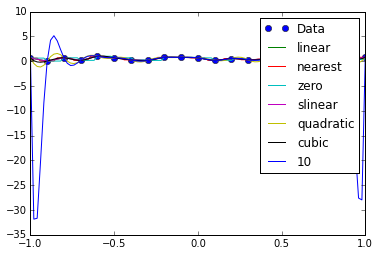
\includegraphics[width=10cm]{1}
 \caption{Errores relativos utilizando la serie de potencias \cite{P}.}
\end{figure}

Tomando como referencia a la figura 1, se realizó un código en Python, similar al utilizado en la Actividad 6, para poder crear una gráfica comparando los errores relativos dependiendo de qué tanta exactitud le des a \eqref{T}, con los términos agregados en su serie de potencias. \\

Al estar realizando el código, no pude crear una representación exacta de la figura 1, por lo que se presenta el programa realizado y la gráfica con mayor aproximación obtenida.

\subsection*{Programa: Comparando errores relativos}

{\color{RoyalPurple}\begin{verbatim}
#Bibliotecas utilizadas
from scipy.integrate import quad
import numpy as np
import matplotlib.pyplot as plt

#------------------------------------------
#Definimos las constantes 
#Valor de la gravedad
g=9.8        
#Longitud de la cuerda
l=0.5  
#Periodo base
T0=2*np.pi*np.sqrt(l/g)
#Que tan tupido esta el intervalo
n=1000

#Error añadido para que no divida entre 0
e=0.0001
#Rango de theta0 
theta0=np.linspace(e,(np.pi)+e,n) 

#------------------------------------------
#Defino los arrays para todos los resultados arrojados
S=[0 for i in range(n)]
TT=[0 for i in range(n)]
R=[0 for i in range(n)]
T=[0 for i in range(n)]
real0=[0 for i in range(n)]
real2=[0 for i in range(n)]
real4=[0 for i in range(n)]
real6=[0 for i in range(n)]
real8=[0 for i in range(n)]

#------------------------------------------
#Con un doble loop para poder considerar los casos
#donde se agregan mas terminos de la serie de potencias

#Paso a paso con los términos porque no se hacer multigraficas
M0=0

#Comienzo un loop para poder calcular todos los resultados 
#posibles contemplando un angulo inicial variante
for i in range(M0):
    for j in range(0,n):
        F1=float(math.factorial(2*i))
        F2=float(((2**i)*(math.factorial(i)))**2)
        
        S[j]=np.sin(theta0[j]/2)**(2*i)
        TT[j]=((F1/F2)**2)*(S[j])
        R[j]=TT[j]+R[j]
        T[j]=R[j]*T0
        real0[j]=(T[j]/T0)
#------------------------------------------        
M2=2
for i in range(M2):
    for j in range(0,n):
        F1=float(math.factorial(2*i))
        F2=float(((2**i)*(math.factorial(i)))**2)
        
        
        S[j]=np.sin(theta0[j]/2)**(2*i)
        TT[j]=((F1/F2)**2)*(S[j])
        R[j]=TT[j]+R[j]
        T[j]=R[j]*T0
        real2[j]=(T[j]/T0)-1
#------------------------------------------        
M4=4
for i in range(M4):
    for j in range(0,n):
        F1=float(math.factorial(2*i))
        F2=float(((2**i)*(math.factorial(i)))**2)
        
        S[j]=np.sin(theta0[j]/2)**(2*i)
        TT[j]=((F1/F2)**2)*(S[j])
        R[j]=TT[j]+R[j]
        T[j]=R[j]*T0
        real4[j]=(T[j]/T0)-2
#------------------------------------------
M6=6
for i in range(M6):
    for j in range(0,n):
        F1=float(math.factorial(2*i))
        F2=float(((2**i)*(math.factorial(i)))**2)
        
        S[j]=np.sin(theta0[j]/2)**(2*i)
        TT[j]=((F1/F2)**2)*(S[j])
        R[j]=TT[j]+R[j]
        T[j]=R[j]*T0
        real6[j]=(T[j]/T0)-3
#------------------------------------------
M8=8
for i in range(M8):
    for j in range(0,n):
        F1=float(math.factorial(2*i))
        F2=float(((2**i)*(math.factorial(i)))**2)
        
        S[j]=np.sin(theta0[j]/2)**(2*i)
        TT[j]=((F1/F2)**2)*(S[j])
        R[j]=TT[j]+R[j]
        T[j]=R[j]*T0
        real8[j]=(T[j]/T0)-4



#------------------------------------------
#Para la grafica
plt.plot(theta0, real0, 'y', label="T0")
plt.plot(theta0, real2, 'm', label="T2")
plt.plot(theta0, real4, 'r', label="T4")
plt.plot(theta0, real6, 'b', label="T6")
plt.plot(theta0, real8, 'g', label="T8")
plt.title('Error using power series')
plt.grid()
plt.xlabel('Angle')
plt.xlim(0,np.pi)
plt.ylabel('Error')
plt.legend(loc='best')

#Pa' guardar la foto sin problemas
fig = matplotlib.pyplot.gcf()
fig.set_size_inches(10.5,5.5)
fig.savefig('error.png',dpi=100)
\end{verbatim}}

\subsection*{Analizando la gráfica obtenida}
\begin{figure}[H]
\centering
\includegraphics[width=15cm]{error}
\caption{Comparando errores dependiendo de los términos en la serie de potencias.}
\end{figure}

\section{Reescribiendo la expresión con Maclaurin}
Reescribiendo a \eqref{T} con la sustitución de la serie Maclaurin de $\displaystyle \sin{\frac{\theta_0}{2}}$, se presenta la mayor aproximacón obtenida con Maxima:\\
\noindent
\begin{minipage}[t]{8ex}{\color{red}\bf
\begin{verbatim}
(%i13) 
\end{verbatim}}
\end{minipage}
\begin{minipage}[t]{\textwidth}{\color{blue}
\begin{verbatim}
S: sin(%theta/2);
\end{verbatim}}
\end{minipage}
\begin{math}\displaystyle
\parbox{8ex}{\color{labelcolor}(\%o13) }
\mathrm{sin}\left( \frac{\theta}{2}\right) 
\end{math}

\noindent
\begin{minipage}[t]{8ex}{\color{red}\bf
\begin{verbatim}
(%i14) 
\end{verbatim}}
\end{minipage}
\begin{minipage}[t]{\textwidth}{\color{blue}
\begin{verbatim}
sS: taylor(S, %theta, 0, 8);
\end{verbatim}}
\end{minipage}
\begin{math}\displaystyle
\parbox{8ex}{\color{labelcolor}(\%o14)}
\frac{\theta}{2}-\frac{{\theta}^{3}}{48}+\frac{{\theta}^{5}}{3840}-\frac{{\theta}^{7}}{645120}+...
\end{math}

\noindent
\begin{minipage}[t]{8ex}{\color{red}\bf
\begin{verbatim}
(%i20) 
\end{verbatim}}
\end{minipage}
\begin{minipage}[t]{\textwidth}{\color{blue}
\begin{verbatim}
mlT: subst(sS, S, T(theta));
\end{verbatim}}
\end{minipage}
\begin{math}\displaystyle
\parbox{8ex}{\color{labelcolor}(\%o20)}
2\,\pi \,\sqrt{\frac{l}{g}}-\frac{\left( {\pi }^{9}-72\,{\pi }^{7}+3024\,{\pi }^{5}-60480\,{\pi }^{3}\right) \,\sqrt{\frac{l}{g}}\,{\theta}^{2}}{2903040}+\cdots
\end{math}

\begin{thebibliography}{6}

\bibitem{W}
Wikipedia,
\emph{Pendulum}. Recuperado en abril de 2016 de \url{https://en.wikipedia.org/wiki/Pendulum\_(mathematics)}

\bibitem{P}
Ferreira, R.
\emph{Pendulum Rel Error90a}. Recuperado en mayo de 2016 de \url{https://en.wikipedia.org/wiki/File:Pendulum_Rel_Error90a.png}

\bibitem{FC}
Lizárraga, C.
\emph{Actividad 9 (2016-1)}. Recuperado en abril de 2016 de \url{http://computacional1.pbworks.com/w/page/106821012/Actividad\%209\%20(2016-1)}

\end{thebibliography}

\end{document}

